The people that use a system can be represented by personas. This is done in order to ensure the PACT elements are centered in the design process\kanote{Hvad menes der her?}. Personas are general profiles of different types of users. A persona is a concrete representation of a fictitious person. Personas help the designer by having a specific end user in mind, preventing them designing the system for themselves. Personas are developed through the understanding process and through undertaking a PACT analysis. A part of the persona is a short story of the person trying to achieve a goal using the system in a specific context~\cite{benyon2013designing}.

As part of this project, three personas was made. The personas was made by following the 10 step process described in~\cite{lene2007persona}.

Here is a description of each of the step and how they were conducted in this project. In some of the steps there will be used a slightly different approach since there did not exist product at the time the personas was made. This mean the personas will be about potential users using a potential system.

\frnote{advarsel brug af you over det hele}
\subsubsection{Step 1: Finding the Users}
In this step general information about the users as a group is gathered. It should be determined how many users there are and in which way they will be using the product. This is done by gathering quatavia data from interviews, observation or questionnaires. When the persona creation process started there were some knowledge some information about the users from observational data. There was also information from the interviews to help getting to know our users better. This resulted in a summary found in~\cref{userInterviews}

\subsubsection{Step 2: Building a Hypothesis}
In this step it is analysed how the users are different and they are put into different groups. This is done using the material gathered in step 1. Initially there was looked at 2 overall groups: bartenders and the users of the app.

\subsubsection{Step 3: Verification}
In verification the focus is on finding data that supports the initial patterns found in step 3. This will later support the personas descriptions and the scenario writing. This is also the step where you go more in depth with the users. What do they dislike, what are their values, what are their attitudes towards the system/site, in what conditions will they use the system/site? This data is then compared to the data from step 3. To find any potential flaws or new groups of users.

After doing this step it was found that there were 2 kind of user: the ones that already did music requesting and the ones that did not.

\subsubsection{Step 4: Finding Patterns}
This is where you categorise the users based on the initial separation from step 2. Are the groups right?

After this step there were three distinct groups:
\begin{enumerate}
\item Bartenders
\item Introvert users \frnote{skal have et bedre navn}
\item Extrovert users
\end{enumerate}

\subsubsection{Step 5: Constructing Personas}
This is the step where the actual personas are made. Based on the patterns found in step 4 one persona representing each group are made. This is done with narrative techniques to tell a story about a person. It is important not to come up with stereotypes, but with realistic person that people can relate to. Some information is based on actual data while other information can be made up to fill in the gaps. According to~\cite{lene2007persona} it is important that as many people are involved in the process of creating personas. The personas for the project was done as a collaboration between the whole group. The three resulting personas can be seen in \cref{akkpersona}.

\subsubsection{Step 6: Defining Situations}
In this step you take each of the personas from step 5 and look at they needs and find out in what situations they will use the product.

\frnote{what we did}

\subsubsection{Step 7: Validation and Buy-in}
In this step the personas are validated by someone not involved in the creation process. This will result in a list of corrections. In this project a person not involved got to read the personas and give comments, this lead to mirror adjustments.

\subsubsection{Step 8: Dissemination of Knowledge}
In this step you have to consider how to get the information from the personas out the the developers and designers that needs to use them. Since this project is done by a small group this was not a big problem. The personas was printed out and places in our workspace, so that they would be easy accessible for everyone.

\subsubsection{Step 9: Creating Scenarios}
In this step it is described what happens when a user uses the product with a goal in mind. This will be based on the persona from step 5 and situations from from step 6. The resulting persona with scenario can be seen in \cref{akkpersona}. This step will also result in use cases in this project the use cases can be found in \cref{usecase}.

\subsubsection{Step 10: Ongoing Development}
The last step is an ongoing step where you update the information if needed. This can happen when there is new data showing something not consider before. The personas for this project only got minor updates along the way.

\subsection{Personas used in the projekt}\label{akkpersona}

\subsubsection{Camilla}
\begin{figure} [h]
  \centering
  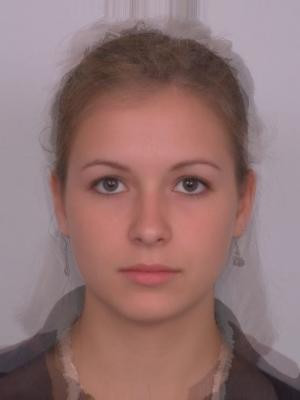
\includegraphics[]{Images/camilla.jpg}
  \caption{Picture associated with the persona \enquote{Camilla}. Copyright the Face Research Lab. Used with permission.}
  \label{fig:camilla}
\end{figure}
\noindent\textbf{Basic information}
\begin{itemize}
\item 20 years old
\item Medical student
\item Employed in an elderly care center
\item In a relationship with Keith
\item She loves meeting new people
\item When going out she likes to visit small places that allow socialisation
\item Volunteered in Red Cross Uganda
\end{itemize}

It is Friday afternoon and Camilla is planning to meet some of her fellow students at a bar. Camilla and her friends get together after they are finished at school and go to a café to grab a sandwich. After dinner, Camilla takes out her smartphone and checks openPlaylist. Camilla can see that some of her favourite tracks are being played at White Hart, and they agree to go there. Upon arriving Camilla checks in via the application. She immediately notices on the screen behind the bar that the queue is filled with tracks she dislikes. She now uses the application to request and upvote other tracks that she would like to be played. Some other people at White Hart agree on Camilla's choices and they too upvote these tracks. On the screen in the bar Camilla can see some of the other people that upvotes her tracks and later in the evening she meets them and they talk about all the nice music they have in common. Camilla and her new and old friends party all night long and drink a lot of beer.

\subsubsection{Adam}
\begin{figure} [h]
  \centering
  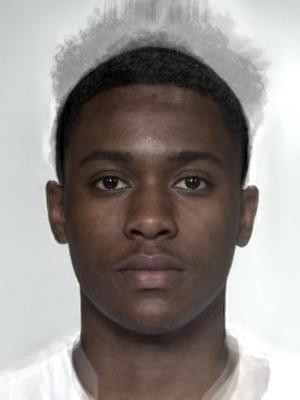
\includegraphics[]{Images/adam.jpg}
  \caption{Picture associated with the persona \enquote{Adam}. Copyright the Face Research Lab. Used with permission.}
  \label{fig:adam}
\end{figure}
\noindent\textbf{Basic information}
\begin{itemize}
\item 23 years old
\item Extrovert
\item Works as an instructor at a fitness center and as an bartender in the weekends
\item Likes socialising and talking to people
\end{itemize}

\subsubsection{Mathias}
\begin{figure} [h]
  \centering
  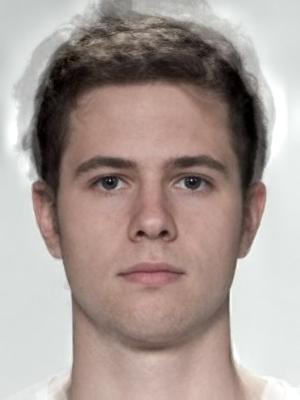
\includegraphics[]{Images/mathias.jpg}
  \caption{Picture associated with the persona \enquote{Mathias}. Copyright the Face Research Lab. Used with permission.}
  \label{fig:mathias}
\end{figure}
\noindent\textbf{Basic information}
\begin{itemize}
\item 21 years old
\item Mechanical engineering student
\item Introvert
\item Thoughtful person that can be shy at times
\end{itemize}
